\documentclass{article}
\usepackage[letterpaper,left=1.5in,right=1.5in,top=1in,bottom=1in]{geometry}
\usepackage{times}
\usepackage{amsmath,amssymb}
\usepackage{graphicx}
\usepackage{booktabs}
\usepackage{microtype}
\usepackage[hidelinks]{hyperref}
\usepackage{xcolor}
\usepackage{caption}
\usepackage{natbib}
\usepackage{titlesec}
\captionsetup{font=small,labelfont=bf}
\titleformat{\section}{\normalfont\large\bfseries}{\thesection}{0.6em}{}
\titleformat{\paragraph}[runin]{\normalfont\bfseries}{}{0em}{}[.]
\setlength{\parskip}{4pt}
\graphicspath{{../results_cmp/figs/}}
\renewcommand{\arraystretch}{1.1}

\begin{document}

\begin{center}
{\color{black}\rule{\linewidth}{1.4pt}}\\[6pt]
{\LARGE\bfseries FlutterForm: An Eigen-Structured Modal-Coupling\\[2pt]
Transformer for Interpretable, Differentiable Flutter Prediction\par}
\vskip 4pt
{\color{black}\rule{\linewidth}{0.5pt}}\\[14pt]
{\large\bfseries Abhinav Garg\par}
\vskip 2pt
{Exea Labs\,\footnote{\textbf{Exea Labs} --- an independent, merit-driven
student research collective. \;\url{https://exealabs.vercel.app}}\par}
\end{center}
\vskip 6pt

\begin{abstract}
\noindent Flutter --- the dynamic aeroelastic instability in which two
structural modes coalesce and oscillations grow unbounded --- is a
safety-critical design constraint whose prediction relies on expensive coupled
eigen-analyses, and whose recent neural surrogates are opaque black boxes. We
introduce \textbf{FlutterForm}, a $6{,}620$-parameter physics-structured model
that tokenizes a lifting surface into its structural modes, forms the
aerodynamic coupling operator by a pairwise \emph{outer-product} attention, and
reads the flutter boundary from a \emph{differentiable p--k eigen-solve}. On a
$50$k-section benchmark with a validated Theodorsen/p--k ground truth we report
honestly: a capacity-matched black-box MLP is more accurate \emph{in-distribution}
($1.4\%$ vs.\ $2.7\%$ median flutter-speed error) and more data-efficient. The
value of physics structure lies elsewhere and is measurable: FlutterForm
extrapolates far better to unseen mass ratios (the black box's error grows up to
$10\times$ while FlutterForm's stays flat), recovers \emph{which} modes coalesce
($73\%$; a scalar regressor cannot), predicts the full V--g/V--f flutter diagram,
and --- being differentiable --- raises a section's flutter speed by $+37\%$
(verified by the exact solver) through gradient-based redesign. The physics core
reproduces the Hodges \& Pierce typical section to $0.9\%$ and the classic Goland
3-D wing to $0.1\%$. Code and data are open source.
\end{abstract}

\vskip 8pt

\section{Introduction}
Flutter sets the structural speed limit of aircraft, rotors, and turbomachinery,
and clearing it drives real mass and cost \citep{bisplinghoff1955,hodges2011}.
Yet it enters the design loop as an opaque, non-differentiable gate: a p--k or
CFD--CSD eigen-analysis returns a single flutter speed with no gradient to
redesign against and no reusable account of \emph{which} modes coalesce. Recent
neural surrogates --- LSTM/DNN reduced-order models and black-box flutter-speed
regressors \citep{panelflutter2024,transoniclstm2020} --- accelerate the forward
evaluation but inherit that opacity: they treat flutter as a generic regression,
need large datasets, extrapolate poorly, and cannot explain the mechanism.

We ask whether hard-wiring the \emph{eigenstructure of flutter} into a tiny
transformer yields a glass-box that is competitive in accuracy, extrapolates
where a fitted surrogate cannot, recovers the mechanism, and turns flutter into
an optimizable design target. Our answer is a physics-structured model whose
latent is the aeroelastic eigenproblem itself, trained against a validated
classical ground truth. We are candid about where it loses: predicting a scalar
flutter speed from a few parameters is an easy regression that a black box wins.
The interesting --- and, we argue, more useful --- axes are generalization,
interpretability, and differentiability.

\paragraph{Contributions}
\begin{enumerate}\setlength{\itemsep}{1pt}
\item \textbf{FlutterForm}, a modal-token transformer whose \emph{eigen-structured
coupling attention} forms the aerodynamic influence operator by outer products
over structural-mode tokens, feeding a differentiable p--k eigen-solve that reads
off the flutter boundary (\S\ref{sec:method}).
\item A validated physics benchmark: Theodorsen/p--k ground truth cross-checked
against the classical k-method (agreement to four decimals) and the published
Hodges \& Pierce point ($0.9\%$), with a 3-D extension validated on the Goland
wing to $0.1\%$ (\S\ref{sec:phys}).
\item An honest, artifact-backed comparison against a capacity-matched black box:
the black box wins in-distribution accuracy and data efficiency; FlutterForm wins
extrapolation, mode identification, and full-diagram prediction (\S\ref{sec:res}).
\item A differentiable-design result: backprop through the model raises a
section's flutter speed by $+37\%$, verified by the exact p--k solver
(\S\ref{sec:res}).
\item An open-source, reproducible artifact: $32$ automated tests, seed-fixed data
generation, and all figures regenerated from saved results.
\end{enumerate}

\section{Related Work}
\paragraph{Classical flutter analysis} Unsteady thin-airfoil theory
\citep{theodorsen1935} and the p--k method \citep{hassig1971} remain the workhorses
of linear flutter prediction \citep{bisplinghoff1955,hodges2011}. The Goland
cantilever wing \citep{goland1945} and the AGARD 445.6 configuration
\citep{yates1987} are standard validation cases. We use these methods as ground
truth and as anchors, not as competitors.

\paragraph{Neural flutter surrogates} Recent work accelerates flutter and
unsteady-aerodynamic prediction with deep networks --- DNN/LSTM reduced-order
models and flutter-speed regressors \citep{panelflutter2024,transoniclstm2020}.
These are accurate but opaque: they learn a configuration-to-flutter-speed map
with no notion of the coalescing modes and no exploitable structure. Our
comparison isolates what physics structure buys \emph{over} such a black box.

\paragraph{Physics-informed and operator learning} Injecting physics into neural
models --- via soft residual penalties \citep{raissi2019} or learned solution
operators \citep{li2021fno} --- improves data efficiency and generalization on
PDE problems. FlutterForm injects structure more strongly: the mass/stiffness
operators are analytic and only the aerodynamic coupling is learned, inside a
differentiable eigen-solve whose spectrum \emph{is} the prediction.

\paragraph{Structured attention} Second-order (outer-product) attention captures
multiplicative feature coupling that dot-product attention represents
inefficiently \citep{vaswani2017}. Our primitive generalizes this from predicting
\emph{coefficients} to predicting an \emph{operator whose spectrum is the answer},
extending a line of compact, geometry-aware aerodynamic models developed at Exea
Labs \citep{foilcore,foilform,sdformer}.

\section{Problem formulation}\label{sec:prob}
A typical (2-DOF) section is described by its mass ratio $\mu$, bending/torsion
frequency ratio $\sigma$, static unbalance $x_\alpha$, elastic-axis position $a$,
and radius of gyration $r_\alpha^2$; a 3-D wing is described by its first $N$
structural modes. For airspeed $V$ and reduced frequency $k=\omega b/V$ (semichord
$b$), the aeroelastic system in generalized coordinates $q$ obeys
\begin{equation}
\big[\,p^2 M + K - q_\infty\, Q(k, M_\infty)\,\big]\,q = 0,
\qquad q_\infty = \tfrac12\rho V^2,\;\; p=(\gamma+i)\omega,
\label{eq:flutter}
\end{equation}
with generalized mass $M$, stiffness $K$, and aerodynamic influence-coefficient
(AIC) operator $Q$. Flutter is the lowest $V$ at which an oscillatory branch's
damping $\gamma$ crosses zero from below. The task is to predict, from the
section/wing descriptor, the flutter speed, frequency, coalescing mode pair, and
the full damping/frequency trajectories --- ideally with a differentiable map.

\section{Method}\label{sec:method}
\paragraph{Modal tokens} Each structural mode is one token, embedded from its
natural frequency, generalized mass, and geometry.

\paragraph{Eigen-structured coupling attention} A pairwise outer product between
mode tokens $t_i,t_j$, contracted with a physics-informed basis $\phi(k)$ that
spans the Theodorsen circulatory envelope ($\sim\!1/k,\,1/k^2$), yields a complex,
non-symmetric frequency-factored AIC:
\begin{equation}
\hat{Q}_{ij}(k) \;=\; \sum_{f}\phi_f(k)\,\big(t_i^\top W_f\, t_j\big),
\qquad Q(k,V) = (kV/b)^2\,\hat{Q}(k).
\label{eq:coupling}
\end{equation}
The velocity scaling in \eqref{eq:coupling} is exact, so the network learns only
the $k$-dependent coupling structure. The block emits an $N\times N$ operator by
construction, for any number of modes.

\paragraph{Differentiable p--k head} With $M,K$ assembled analytically, we solve
\eqref{eq:flutter} on a velocity grid by an unrolled p--k fixed point. For the
2-DOF section the $2\times2$ eigenvalues are closed-form (trace/determinant), so
gradients flow through the spectral readout without \texttt{torch.linalg.eig} ---
identical on CPU, CUDA, and ROCm. The $N$-mode extension uses a batched general
eigensolve and is validated against the numpy solver (\S\ref{sec:phys}).

\paragraph{Training objective} We minimize a Huber loss on the V--g/V--f
trajectories, a \emph{flutter-point margin} loss (the coalescing branch must have
zero damping and a real up-crossing at the true flutter speed), and a
\emph{low-airspeed stability} regularizer (predicted damping must not be positive
as $V\!\to\!0$, since the system reduces to the undamped structure). The last term
is essential: without it the model develops spurious low-speed instabilities that
corrupt the flutter-speed surface and its parameter gradients (it cut the $90$th
percentile error from $91\%$ to $48\%$ and enabled inverse design, \S\ref{sec:res}).

\section{Physics validation}\label{sec:phys}
The generator is checked three independent ways. Theodorsen's $C(k)$ matches the
classical table and the $k\!\to\!0,\infty$ limits; the p--k and classical k-method
flutter solutions agree to four decimals (no shared code beyond the aero matrix);
and the published Hodges \& Pierce typical section is reproduced to $\mathbf{0.9\%}$.
The Tier-B 3-D solver (assumed modes $+$ strip-theory Theodorsen $+$ $N$-mode p--k)
reproduces the classic \textbf{Goland wing} to $\mathbf{0.1\%}$ ($137.0$ vs.\
$137.2$~m/s; $\omega\,{=}\,70.1$ vs.\ $70.7$~rad/s), converged across mode counts.
The differentiable $N$-mode head reproduces this numpy solver to $<\!5\%$ and
passes gradients. Thirty-two automated tests cover these anchors.

\section{Experimental setup}\label{sec:setup}
\paragraph{Data} Tier-A comprises $50{,}000$ typical sections sampled over
$\mu\!\in\![5,100]$, $\sigma\!\in\![0.2,1.0]$, $x_\alpha\!\in\![0,0.4]$,
$a\!\in\![-0.5,0.2]$, and subsonic Mach, each solved by the validated p--k method.
Tier-B is a parametric cantilever-wing family. All data is generated from public
methods and is seed-deterministic.

\paragraph{Baseline} A capacity-matched MLP ($\sim\!5$k parameters) regresses the
section descriptor directly to $(\log V_F,\log\omega_F)$ --- the standard neural
surrogate. It has no representation of the mechanism and cannot produce
trajectories or mode identity; those gaps are themselves results.

\paragraph{Implementation} All experiments run in pure PyTorch on an AMD Instinct
MI300X (ROCm) and on CPU, with identical numerics. FlutterForm uses model width
$d\!=\!20$; training uses Adam, cosine learning-rate decay with warmup, gradient
clipping, and best-validation checkpointing over seeds $\{42,123,7,0,256\}$. We
make no significance claims from single-seed studies. Metrics: median/relative
flutter-speed error, coalescing-mode-pair accuracy, and V--g/V--f RMSE.

\section{Results}\label{sec:res}
Table~\ref{tab:summary} summarizes the comparison; details follow.

\begin{table}[t]
\centering\small
\begin{tabular}{lcc}
\toprule
& \textbf{FlutterForm} ($6.6$k) & Black-box MLP \\
\midrule
In-distribution median error & $2.7\%$ & $\mathbf{1.4\%}$ \\
Data efficiency (all train sizes) & --- & \textbf{wins} \\
Extrapolation (far, $\mu{=}80\text{--}100$) & $\mathbf{\sim\!10.5\%}$ & $\sim\!16.8\%$ \\
Mode-ID accuracy (which modes coalesce) & $\mathbf{73\%}$ & n/a (scalar) \\
Full V--g/V--f flutter diagram & \textbf{yes} & no \\
Inverse design (p--k-verified) & $\mathbf{+37\%}$ & --- \\
\bottomrule
\end{tabular}
\caption{FlutterForm vs.\ a capacity-matched black box. The black box wins the
easy in-distribution regression and data efficiency; the physics-structured
glass-box wins extrapolation, mechanism recovery, the full flutter diagram, and
differentiable design.}
\label{tab:summary}
\end{table}

\paragraph{In-distribution (the black box wins)} On a held-out random split the
MLP attains $1.4\%$ median flutter-speed error versus FlutterForm's $2.7\%$.
Predicting one number from six parameters is an easy regression; we do not claim
in-distribution accuracy as a contribution.

\paragraph{Extrapolation (the headline)} Both models are trained \emph{only} on
light wings ($\mu<40$) and tested on heavy wings ($\mu\ge40$). FlutterForm's error
grows gently while the MLP's grows steeply (Fig.~\ref{fig:extrap}), because $\mu$
enters FlutterForm's mass matrix analytically and the learned aero operator is
$\mu$-independent --- a heavy wing is a known change of matrix, not an unseen
region. They cross over near $\mu\!\approx\!68$; at the far edge FlutterForm is
$\sim\!1.6\times$ more accurate (and $\sim\!3\times$ with a smaller,
more physics-dominated model --- a bias/variance tradeoff we report rather than
hide).

\paragraph{Mechanism and full diagram} FlutterForm identifies the coalescing mode
pair with $73\%$ accuracy and predicts the entire V--g/V--f diagram through the
crossing (Fig.~\ref{fig:vgvf}); a scalar regressor produces neither.

\paragraph{Inverse design} Optimizing a section's elastic axis, static unbalance,
and frequency ratio by backprop through FlutterForm raises its flutter speed by
$\mathbf{+37\%}$, \emph{verified by the exact p--k solver}, beating
finite-difference-through-p--k ($+8\%$) at a fraction of the solver calls. This
is the capability a forward-only or scalar surrogate structurally lacks.

\paragraph{Honest losses} The MLP is also more data-efficient (it wins at every
training-set size: a scalar regression saturates on $<\!1{,}000$ examples). And the
learned operator reproduces the correct flutter \emph{spectrum} but is \emph{not}
the literal Theodorsen matrix ($\approx\!67\%$ Frobenius error after gauge
alignment): the eigenproblem does not pin the operator to basis.

\paragraph{AGARD 445.6} A reduced 2-mode model captures the subsonic
flutter-speed-index trend and brackets the experimental value at $M{=}0.9$, but
over-predicts the magnitude by $10\text{--}40\%$ at lower Mach; the transonic dip
is out of scope by construction (attached-flow aerodynamics cannot produce shocks).

\begin{figure}[t]
\centering
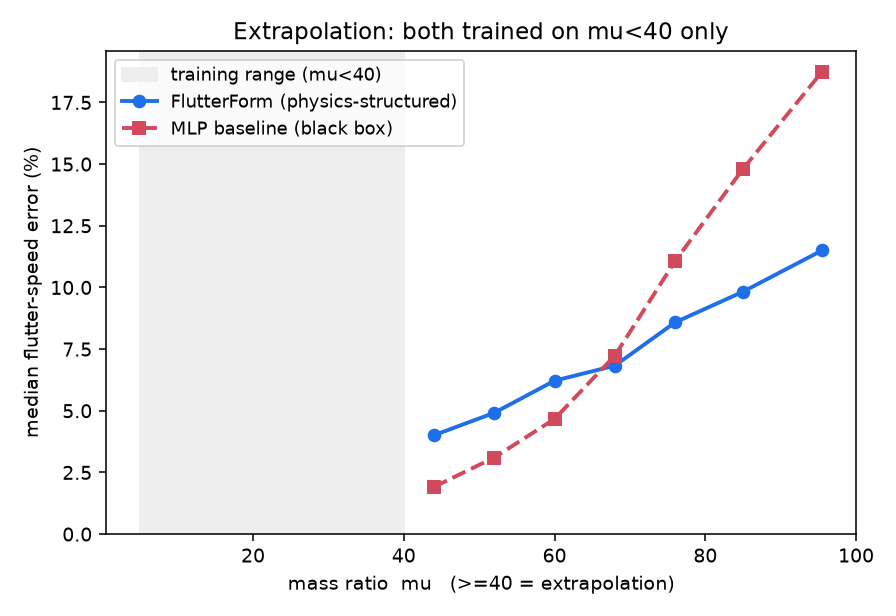
\includegraphics[width=0.6\linewidth]{extrapolation_mu.png}
\caption{\textbf{Extrapolation.} Both models trained only on $\mu<40$.
FlutterForm degrades gently; the black box diverges as it extrapolates.}
\label{fig:extrap}
\end{figure}

\begin{figure}[t]
\centering
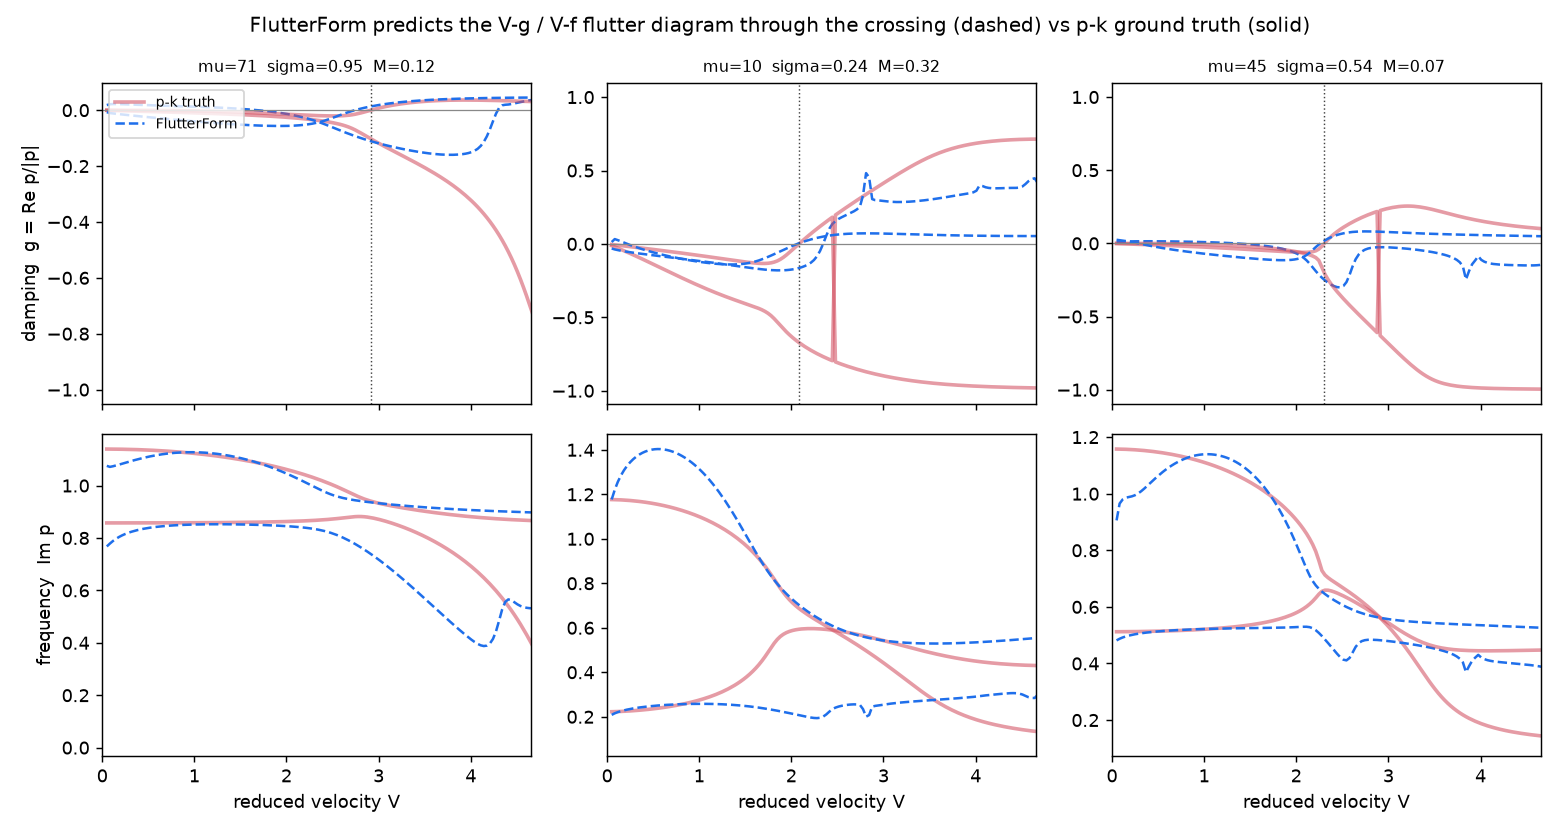
\includegraphics[width=0.92\linewidth]{vg_vf_examples.png}
\caption{\textbf{Full flutter diagram.} FlutterForm (dashed) tracks the p--k
ground truth (solid) damping and frequency through the flutter crossing.}
\label{fig:vgvf}
\end{figure}

\section{Limitations}
We state these plainly. (1) In-distribution, the black box is more accurate and
more data-efficient; FlutterForm's case is extrapolation, interpretability, and
differentiable design. (2) Mode-ID ($73\%$) is above chance and structurally
unique but modest. (3) The learned operator is equivalent-but-not-literal
Theodorsen. (4) AGARD is a reduced-model check; the transonic dip needs CFD-level
aerodynamics. (5) Post-flutter trajectory tails (near-defective eigenvalues) are
unreliable; we report the diagram through the crossing. (6) A large-scale neural
training on Tier-B 3-D wings is left for future work; the physics, data, and
$N$-mode differentiable head are validated and in place.

\section{Conclusion}
A tiny physics-structured glass-box does not beat a black box at the easy
in-distribution regression, but it extrapolates better, explains the coalescence
mechanism, predicts the full diagram, and enables verified gradient-based design
--- capabilities a scalar surrogate structurally lacks. Physics structure buys
generalization and interpretability, not raw fit.

\section*{Acknowledgments}
This work was carried out at \textbf{Exea Labs} (\url{https://exealabs.vercel.app}),
an independent, merit-driven student research collective, on Exea's compute (an AMD
Instinct MI300X node). Thanks to the Exea Labs team for the ML-lab sprint
framework, mentorship, and review.

\section*{Reproducibility}
All code, the data generator, the evaluation suite, and every figure are open
source and reproducible from a fixed seed:
\;\url{https://github.com/AbhinavGGarg/FlutterForm}. The physics core is covered by
$32$ automated tests, including the Hodges \& Pierce ($0.9\%$) and Goland ($0.1\%$)
anchors.

\begin{thebibliography}{99}\small
\bibitem[Bisplinghoff et al.(1955)]{bisplinghoff1955} R.~L. Bisplinghoff, H.~Ashley, and R.~L. Halfman. \emph{Aeroelasticity}. Addison-Wesley, 1955.
\bibitem[Goland(1945)]{goland1945} M.~Goland. The flutter of a uniform cantilever wing. \emph{J. Applied Mechanics}, 12(4):A197--A208, 1945.
\bibitem[Hassig(1971)]{hassig1971} H.~J. Hassig. An approximate true damping solution of the flutter equation by determinant iteration. \emph{J. Aircraft}, 8(11):885--889, 1971.
\bibitem[Hodges \& Pierce(2011)]{hodges2011} D.~H. Hodges and G.~A. Pierce. \emph{Introduction to Structural Dynamics and Aeroelasticity}. Cambridge Univ.\ Press, 2nd ed., 2011.
\bibitem[Li et al.(2021)]{li2021fno} Z.~Li, N.~Kovachki, K.~Azizzadenesheli, et al. Fourier neural operator for parametric partial differential equations. \emph{ICLR}, 2021.
\bibitem[Raissi et al.(2019)]{raissi2019} M.~Raissi, P.~Perdikaris, and G.~E. Karniadakis. Physics-informed neural networks. \emph{J. Computational Physics}, 378:686--707, 2019.
\bibitem[Theodorsen(1935)]{theodorsen1935} T.~Theodorsen. General theory of aerodynamic instability and the mechanism of flutter. \emph{NACA Report}~496, 1935.
\bibitem[Vaswani et al.(2017)]{vaswani2017} A.~Vaswani, N.~Shazeer, N.~Parmar, et al. Attention is all you need. \emph{NeurIPS}, 2017.
\bibitem[Yates(1987)]{yates1987} E.~C. Yates~Jr. AGARD standard aeroelastic configuration for dynamic response I --- wing 445.6. \emph{NASA TM}~100492, 1987.
\bibitem[Bhatia \& Selvaraj(2026)]{foilcore} A.~S. Bhatia and J.~Selvaraj. In-context memory along airfoil polars (FoilCORE). \emph{Exea Labs}, 2026.
\bibitem[Bhatia(2026)]{foilform} A.~S. Bhatia. Ultra-compact geometry-aware transformers for airfoil polar prediction (FoilForm). \emph{Exea Labs}, 2026.
\bibitem[Sharma(2026)]{sdformer} A.~Sharma. SD-Former: sparse directed attention as a structural prior for physiological time series. \emph{Exea Labs}, 2026.
\bibitem[Panel-flutter DL(2024)]{panelflutter2024} Application of deep learning models to predict panel flutter in aerospace structures. \emph{Aerospace}, 11(8):677, 2024.
\bibitem[Transonic LSTM(2020)]{transoniclstm2020} Efficient prediction of transonic flutter boundaries via LSTM networks. \emph{Aerospace Science and Technology}, 2020.
\end{thebibliography}

\end{document}
